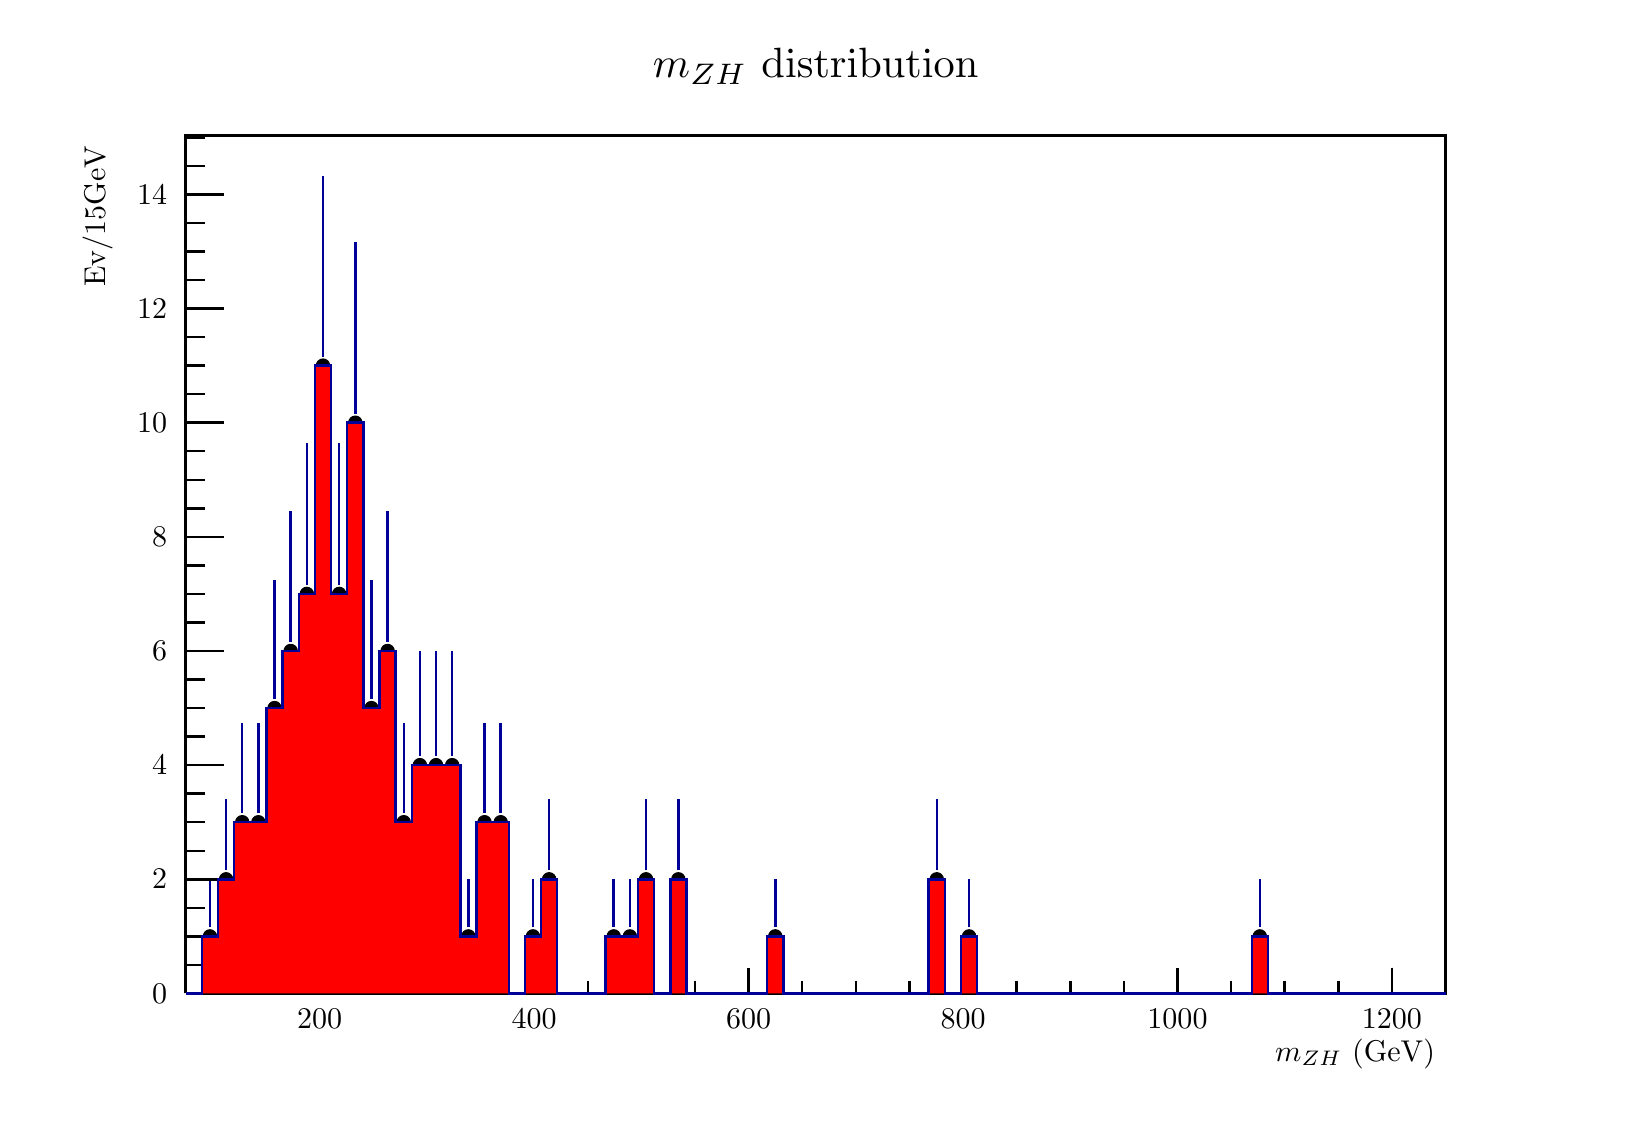
\begin{tikzpicture}
\pgfdeclareplotmark{cross} {
\pgfpathmoveto{\pgfpoint{-0.3\pgfplotmarksize}{\pgfplotmarksize}}
\pgfpathlineto{\pgfpoint{+0.3\pgfplotmarksize}{\pgfplotmarksize}}
\pgfpathlineto{\pgfpoint{+0.3\pgfplotmarksize}{0.3\pgfplotmarksize}}
\pgfpathlineto{\pgfpoint{+1\pgfplotmarksize}{0.3\pgfplotmarksize}}
\pgfpathlineto{\pgfpoint{+1\pgfplotmarksize}{-0.3\pgfplotmarksize}}
\pgfpathlineto{\pgfpoint{+0.3\pgfplotmarksize}{-0.3\pgfplotmarksize}}
\pgfpathlineto{\pgfpoint{+0.3\pgfplotmarksize}{-1.\pgfplotmarksize}}
\pgfpathlineto{\pgfpoint{-0.3\pgfplotmarksize}{-1.\pgfplotmarksize}}
\pgfpathlineto{\pgfpoint{-0.3\pgfplotmarksize}{-0.3\pgfplotmarksize}}
\pgfpathlineto{\pgfpoint{-1.\pgfplotmarksize}{-0.3\pgfplotmarksize}}
\pgfpathlineto{\pgfpoint{-1.\pgfplotmarksize}{0.3\pgfplotmarksize}}
\pgfpathlineto{\pgfpoint{-0.3\pgfplotmarksize}{0.3\pgfplotmarksize}}
\pgfpathclose
\pgfusepathqstroke
}
\pgfdeclareplotmark{cross*} {
\pgfpathmoveto{\pgfpoint{-0.3\pgfplotmarksize}{\pgfplotmarksize}}
\pgfpathlineto{\pgfpoint{+0.3\pgfplotmarksize}{\pgfplotmarksize}}
\pgfpathlineto{\pgfpoint{+0.3\pgfplotmarksize}{0.3\pgfplotmarksize}}
\pgfpathlineto{\pgfpoint{+1\pgfplotmarksize}{0.3\pgfplotmarksize}}
\pgfpathlineto{\pgfpoint{+1\pgfplotmarksize}{-0.3\pgfplotmarksize}}
\pgfpathlineto{\pgfpoint{+0.3\pgfplotmarksize}{-0.3\pgfplotmarksize}}
\pgfpathlineto{\pgfpoint{+0.3\pgfplotmarksize}{-1.\pgfplotmarksize}}
\pgfpathlineto{\pgfpoint{-0.3\pgfplotmarksize}{-1.\pgfplotmarksize}}
\pgfpathlineto{\pgfpoint{-0.3\pgfplotmarksize}{-0.3\pgfplotmarksize}}
\pgfpathlineto{\pgfpoint{-1.\pgfplotmarksize}{-0.3\pgfplotmarksize}}
\pgfpathlineto{\pgfpoint{-1.\pgfplotmarksize}{0.3\pgfplotmarksize}}
\pgfpathlineto{\pgfpoint{-0.3\pgfplotmarksize}{0.3\pgfplotmarksize}}
\pgfpathclose
\pgfusepathqfillstroke
}
\pgfdeclareplotmark{newstar} {
\pgfpathmoveto{\pgfqpoint{0pt}{\pgfplotmarksize}}
\pgfpathlineto{\pgfqpointpolar{44}{0.5\pgfplotmarksize}}
\pgfpathlineto{\pgfqpointpolar{18}{\pgfplotmarksize}}
\pgfpathlineto{\pgfqpointpolar{-20}{0.5\pgfplotmarksize}}
\pgfpathlineto{\pgfqpointpolar{-54}{\pgfplotmarksize}}
\pgfpathlineto{\pgfqpointpolar{-90}{0.5\pgfplotmarksize}}
\pgfpathlineto{\pgfqpointpolar{234}{\pgfplotmarksize}}
\pgfpathlineto{\pgfqpointpolar{198}{0.5\pgfplotmarksize}}
\pgfpathlineto{\pgfqpointpolar{162}{\pgfplotmarksize}}
\pgfpathlineto{\pgfqpointpolar{134}{0.5\pgfplotmarksize}}
\pgfpathclose
\pgfusepathqstroke
}
\pgfdeclareplotmark{newstar*} {
\pgfpathmoveto{\pgfqpoint{0pt}{\pgfplotmarksize}}
\pgfpathlineto{\pgfqpointpolar{44}{0.5\pgfplotmarksize}}
\pgfpathlineto{\pgfqpointpolar{18}{\pgfplotmarksize}}
\pgfpathlineto{\pgfqpointpolar{-20}{0.5\pgfplotmarksize}}
\pgfpathlineto{\pgfqpointpolar{-54}{\pgfplotmarksize}}
\pgfpathlineto{\pgfqpointpolar{-90}{0.5\pgfplotmarksize}}
\pgfpathlineto{\pgfqpointpolar{234}{\pgfplotmarksize}}
\pgfpathlineto{\pgfqpointpolar{198}{0.5\pgfplotmarksize}}
\pgfpathlineto{\pgfqpointpolar{162}{\pgfplotmarksize}}
\pgfpathlineto{\pgfqpointpolar{134}{0.5\pgfplotmarksize}}
\pgfpathclose
\pgfusepathqfillstroke
}
\definecolor{c}{rgb}{1,1,1};
\draw [color=c, fill=c] (0,0) rectangle (20,13.6207);
\draw [color=c, fill=c] (2,1.36207) rectangle (18,12.2586);
\definecolor{c}{rgb}{0,0,0};
\draw [c,line width=0.9] (2,1.36207) -- (2,12.2586) -- (18,12.2586) -- (18,1.36207) -- (2,1.36207);
\definecolor{c}{rgb}{1,1,1};
\draw [color=c, fill=c] (2,1.36207) rectangle (18,12.2586);
\definecolor{c}{rgb}{0,0,0};
\draw [c,line width=0.9] (2,1.36207) -- (2,12.2586) -- (18,12.2586) -- (18,1.36207) -- (2,1.36207);
\definecolor{c}{rgb}{0,0,0.6};
\draw [c,line width=0.9] (2.30769,1.36207) -- (2.30769,1.97199);
\draw [c,line width=0.9] (2.30769,2.20188) -- (2.30769,2.81181);
\definecolor{c}{rgb}{0,0,0};
\foreach \P in {(2.30769,2.08694)}{\draw[mark options={color=c,fill=c},mark size=2.402402pt,mark=*] plot coordinates {\P};}
\definecolor{c}{rgb}{0,0,0.6};
\draw [c,line width=0.9] (2.51282,1.78669) -- (2.51282,2.69686);
\draw [c,line width=0.9] (2.51282,2.92675) -- (2.51282,3.83692);
\definecolor{c}{rgb}{0,0,0};
\foreach \P in {(2.51282,2.81181)}{\draw[mark options={color=c,fill=c},mark size=2.402402pt,mark=*] plot coordinates {\P};}
\definecolor{c}{rgb}{0,0,0.6};
\draw [c,line width=0.9] (2.71795,2.28117) -- (2.71795,3.42173);
\draw [c,line width=0.9] (2.71795,3.65162) -- (2.71795,4.79218);
\definecolor{c}{rgb}{0,0,0};
\foreach \P in {(2.71795,3.53667)}{\draw[mark options={color=c,fill=c},mark size=2.402402pt,mark=*] plot coordinates {\P};}
\definecolor{c}{rgb}{0,0,0.6};
\draw [c,line width=0.9] (2.92308,2.28117) -- (2.92308,3.42173);
\draw [c,line width=0.9] (2.92308,3.65162) -- (2.92308,4.79218);
\definecolor{c}{rgb}{0,0,0};
\foreach \P in {(2.92308,3.53667)}{\draw[mark options={color=c,fill=c},mark size=2.402402pt,mark=*] plot coordinates {\P};}
\definecolor{c}{rgb}{0,0,0.6};
\draw [c,line width=0.9] (3.12821,3.36556) -- (3.12821,4.87147);
\draw [c,line width=0.9] (3.12821,5.10135) -- (3.12821,6.60727);
\definecolor{c}{rgb}{0,0,0};
\foreach \P in {(3.12821,4.98641)}{\draw[mark options={color=c,fill=c},mark size=2.402402pt,mark=*] plot coordinates {\P};}
\definecolor{c}{rgb}{0,0,0.6};
\draw [c,line width=0.9] (3.33333,3.93572) -- (3.33333,5.59634);
\draw [c,line width=0.9] (3.33333,5.82622) -- (3.33333,7.48684);
\definecolor{c}{rgb}{0,0,0};
\foreach \P in {(3.33333,5.71128)}{\draw[mark options={color=c,fill=c},mark size=2.402402pt,mark=*] plot coordinates {\P};}
\definecolor{c}{rgb}{0,0,0.6};
\draw [c,line width=0.9] (3.53846,4.51833) -- (3.53846,6.3212);
\draw [c,line width=0.9] (3.53846,6.55109) -- (3.53846,8.35397);
\definecolor{c}{rgb}{0,0,0};
\foreach \P in {(3.53846,6.43615)}{\draw[mark options={color=c,fill=c},mark size=2.402402pt,mark=*] plot coordinates {\P};}
\definecolor{c}{rgb}{0,0,0.6};
\draw [c,line width=0.9] (3.74359,6.9315) -- (3.74359,9.22068);
\draw [c,line width=0.9] (3.74359,9.45056) -- (3.74359,11.7397);
\definecolor{c}{rgb}{0,0,0};
\foreach \P in {(3.74359,9.33562)}{\draw[mark options={color=c,fill=c},mark size=2.402402pt,mark=*] plot coordinates {\P};}
\definecolor{c}{rgb}{0,0,0.6};
\draw [c,line width=0.9] (3.94872,4.51833) -- (3.94872,6.3212);
\draw [c,line width=0.9] (3.94872,6.55109) -- (3.94872,8.35397);
\definecolor{c}{rgb}{0,0,0};
\foreach \P in {(3.94872,6.43615)}{\draw[mark options={color=c,fill=c},mark size=2.402402pt,mark=*] plot coordinates {\P};}
\definecolor{c}{rgb}{0,0,0.6};
\draw [c,line width=0.9] (4.15385,6.31852) -- (4.15385,8.49581);
\draw [c,line width=0.9] (4.15385,8.72569) -- (4.15385,10.903);
\definecolor{c}{rgb}{0,0,0};
\foreach \P in {(4.15385,8.61075)}{\draw[mark options={color=c,fill=c},mark size=2.402402pt,mark=*] plot coordinates {\P};}
\definecolor{c}{rgb}{0,0,0.6};
\draw [c,line width=0.9] (4.35897,3.36556) -- (4.35897,4.87147);
\draw [c,line width=0.9] (4.35897,5.10135) -- (4.35897,6.60727);
\definecolor{c}{rgb}{0,0,0};
\foreach \P in {(4.35897,4.98641)}{\draw[mark options={color=c,fill=c},mark size=2.402402pt,mark=*] plot coordinates {\P};}
\definecolor{c}{rgb}{0,0,0.6};
\draw [c,line width=0.9] (4.5641,3.93572) -- (4.5641,5.59634);
\draw [c,line width=0.9] (4.5641,5.82622) -- (4.5641,7.48684);
\definecolor{c}{rgb}{0,0,0};
\foreach \P in {(4.5641,5.71128)}{\draw[mark options={color=c,fill=c},mark size=2.402402pt,mark=*] plot coordinates {\P};}
\definecolor{c}{rgb}{0,0,0.6};
\draw [c,line width=0.9] (4.76923,2.28117) -- (4.76923,3.42173);
\draw [c,line width=0.9] (4.76923,3.65162) -- (4.76923,4.79218);
\definecolor{c}{rgb}{0,0,0};
\foreach \P in {(4.76923,3.53667)}{\draw[mark options={color=c,fill=c},mark size=2.402402pt,mark=*] plot coordinates {\P};}
\definecolor{c}{rgb}{0,0,0.6};
\draw [c,line width=0.9] (4.97436,2.81181) -- (4.97436,4.1466);
\draw [c,line width=0.9] (4.97436,4.37648) -- (4.97436,5.71128);
\definecolor{c}{rgb}{0,0,0};
\foreach \P in {(4.97436,4.26154)}{\draw[mark options={color=c,fill=c},mark size=2.402402pt,mark=*] plot coordinates {\P};}
\definecolor{c}{rgb}{0,0,0.6};
\draw [c,line width=0.9] (5.17949,2.81181) -- (5.17949,4.1466);
\draw [c,line width=0.9] (5.17949,4.37648) -- (5.17949,5.71128);
\definecolor{c}{rgb}{0,0,0};
\foreach \P in {(5.17949,4.26154)}{\draw[mark options={color=c,fill=c},mark size=2.402402pt,mark=*] plot coordinates {\P};}
\definecolor{c}{rgb}{0,0,0.6};
\draw [c,line width=0.9] (5.38462,2.81181) -- (5.38462,4.1466);
\draw [c,line width=0.9] (5.38462,4.37648) -- (5.38462,5.71128);
\definecolor{c}{rgb}{0,0,0};
\foreach \P in {(5.38462,4.26154)}{\draw[mark options={color=c,fill=c},mark size=2.402402pt,mark=*] plot coordinates {\P};}
\definecolor{c}{rgb}{0,0,0.6};
\draw [c,line width=0.9] (5.58974,1.36207) -- (5.58974,1.97199);
\draw [c,line width=0.9] (5.58974,2.20188) -- (5.58974,2.81181);
\definecolor{c}{rgb}{0,0,0};
\foreach \P in {(5.58974,2.08694)}{\draw[mark options={color=c,fill=c},mark size=2.402402pt,mark=*] plot coordinates {\P};}
\definecolor{c}{rgb}{0,0,0.6};
\draw [c,line width=0.9] (5.79487,2.28117) -- (5.79487,3.42173);
\draw [c,line width=0.9] (5.79487,3.65162) -- (5.79487,4.79218);
\definecolor{c}{rgb}{0,0,0};
\foreach \P in {(5.79487,3.53667)}{\draw[mark options={color=c,fill=c},mark size=2.402402pt,mark=*] plot coordinates {\P};}
\definecolor{c}{rgb}{0,0,0.6};
\draw [c,line width=0.9] (6,2.28117) -- (6,3.42173);
\draw [c,line width=0.9] (6,3.65162) -- (6,4.79218);
\definecolor{c}{rgb}{0,0,0};
\foreach \P in {(6,3.53667)}{\draw[mark options={color=c,fill=c},mark size=2.402402pt,mark=*] plot coordinates {\P};}
\definecolor{c}{rgb}{0,0,0.6};
\draw [c,line width=0.9] (6.41026,1.36207) -- (6.41026,1.97199);
\draw [c,line width=0.9] (6.41026,2.20188) -- (6.41026,2.81181);
\definecolor{c}{rgb}{0,0,0};
\foreach \P in {(6.41026,2.08694)}{\draw[mark options={color=c,fill=c},mark size=2.402402pt,mark=*] plot coordinates {\P};}
\definecolor{c}{rgb}{0,0,0.6};
\draw [c,line width=0.9] (6.61538,1.78669) -- (6.61538,2.69686);
\draw [c,line width=0.9] (6.61538,2.92675) -- (6.61538,3.83692);
\definecolor{c}{rgb}{0,0,0};
\foreach \P in {(6.61538,2.81181)}{\draw[mark options={color=c,fill=c},mark size=2.402402pt,mark=*] plot coordinates {\P};}
\definecolor{c}{rgb}{0,0,0.6};
\draw [c,line width=0.9] (7.4359,1.36207) -- (7.4359,1.97199);
\draw [c,line width=0.9] (7.4359,2.20188) -- (7.4359,2.81181);
\definecolor{c}{rgb}{0,0,0};
\foreach \P in {(7.4359,2.08694)}{\draw[mark options={color=c,fill=c},mark size=2.402402pt,mark=*] plot coordinates {\P};}
\definecolor{c}{rgb}{0,0,0.6};
\draw [c,line width=0.9] (7.64103,1.36207) -- (7.64103,1.97199);
\draw [c,line width=0.9] (7.64103,2.20188) -- (7.64103,2.81181);
\definecolor{c}{rgb}{0,0,0};
\foreach \P in {(7.64103,2.08694)}{\draw[mark options={color=c,fill=c},mark size=2.402402pt,mark=*] plot coordinates {\P};}
\definecolor{c}{rgb}{0,0,0.6};
\draw [c,line width=0.9] (7.84615,1.78669) -- (7.84615,2.69686);
\draw [c,line width=0.9] (7.84615,2.92675) -- (7.84615,3.83692);
\definecolor{c}{rgb}{0,0,0};
\foreach \P in {(7.84615,2.81181)}{\draw[mark options={color=c,fill=c},mark size=2.402402pt,mark=*] plot coordinates {\P};}
\definecolor{c}{rgb}{0,0,0.6};
\draw [c,line width=0.9] (8.25641,1.78669) -- (8.25641,2.69686);
\draw [c,line width=0.9] (8.25641,2.92675) -- (8.25641,3.83692);
\definecolor{c}{rgb}{0,0,0};
\foreach \P in {(8.25641,2.81181)}{\draw[mark options={color=c,fill=c},mark size=2.402402pt,mark=*] plot coordinates {\P};}
\definecolor{c}{rgb}{0,0,0.6};
\draw [c,line width=0.9] (9.48718,1.36207) -- (9.48718,1.97199);
\draw [c,line width=0.9] (9.48718,2.20188) -- (9.48718,2.81181);
\definecolor{c}{rgb}{0,0,0};
\foreach \P in {(9.48718,2.08694)}{\draw[mark options={color=c,fill=c},mark size=2.402402pt,mark=*] plot coordinates {\P};}
\definecolor{c}{rgb}{0,0,0.6};
\draw [c,line width=0.9] (11.5385,1.78669) -- (11.5385,2.69686);
\draw [c,line width=0.9] (11.5385,2.92675) -- (11.5385,3.83692);
\definecolor{c}{rgb}{0,0,0};
\foreach \P in {(11.5385,2.81181)}{\draw[mark options={color=c,fill=c},mark size=2.402402pt,mark=*] plot coordinates {\P};}
\definecolor{c}{rgb}{0,0,0.6};
\draw [c,line width=0.9] (11.9487,1.36207) -- (11.9487,1.97199);
\draw [c,line width=0.9] (11.9487,2.20188) -- (11.9487,2.81181);
\definecolor{c}{rgb}{0,0,0};
\foreach \P in {(11.9487,2.08694)}{\draw[mark options={color=c,fill=c},mark size=2.402402pt,mark=*] plot coordinates {\P};}
\definecolor{c}{rgb}{0,0,0.6};
\draw [c,line width=0.9] (15.641,1.36207) -- (15.641,1.97199);
\draw [c,line width=0.9] (15.641,2.20188) -- (15.641,2.81181);
\definecolor{c}{rgb}{0,0,0};
\foreach \P in {(15.641,2.08694)}{\draw[mark options={color=c,fill=c},mark size=2.402402pt,mark=*] plot coordinates {\P};}
\draw [c,line width=0.9] (2,1.36207) -- (18,1.36207);
\draw [anchor= east] (18,0.59931) node[scale=1.08496, color=c, rotate=0]{$m_{ZH} \mbox{ (GeV)}$};
\draw [c,line width=0.9] (3.70213,1.68897) -- (3.70213,1.36207);
\draw [c,line width=0.9] (4.38298,1.52552) -- (4.38298,1.36207);
\draw [c,line width=0.9] (5.06383,1.52552) -- (5.06383,1.36207);
\draw [c,line width=0.9] (5.74468,1.52552) -- (5.74468,1.36207);
\draw [c,line width=0.9] (6.42553,1.68897) -- (6.42553,1.36207);
\draw [c,line width=0.9] (7.10638,1.52552) -- (7.10638,1.36207);
\draw [c,line width=0.9] (7.78723,1.52552) -- (7.78723,1.36207);
\draw [c,line width=0.9] (8.46809,1.52552) -- (8.46809,1.36207);
\draw [c,line width=0.9] (9.14894,1.68897) -- (9.14894,1.36207);
\draw [c,line width=0.9] (9.82979,1.52552) -- (9.82979,1.36207);
\draw [c,line width=0.9] (10.5106,1.52552) -- (10.5106,1.36207);
\draw [c,line width=0.9] (11.1915,1.52552) -- (11.1915,1.36207);
\draw [c,line width=0.9] (11.8723,1.68897) -- (11.8723,1.36207);
\draw [c,line width=0.9] (12.5532,1.52552) -- (12.5532,1.36207);
\draw [c,line width=0.9] (13.234,1.52552) -- (13.234,1.36207);
\draw [c,line width=0.9] (13.9149,1.52552) -- (13.9149,1.36207);
\draw [c,line width=0.9] (14.5957,1.68897) -- (14.5957,1.36207);
\draw [c,line width=0.9] (15.2766,1.52552) -- (15.2766,1.36207);
\draw [c,line width=0.9] (15.9574,1.52552) -- (15.9574,1.36207);
\draw [c,line width=0.9] (16.6383,1.52552) -- (16.6383,1.36207);
\draw [c,line width=0.9] (17.3191,1.68897) -- (17.3191,1.36207);
\draw [c,line width=0.9] (3.70213,1.68897) -- (3.70213,1.36207);
\draw [c,line width=0.9] (3.02128,1.52552) -- (3.02128,1.36207);
\draw [c,line width=0.9] (2.34043,1.52552) -- (2.34043,1.36207);
\draw [c,line width=0.9] (17.3191,1.68897) -- (17.3191,1.36207);
\draw [c,line width=0.9] (18,1.52552) -- (18,1.36207);
\draw [anchor=base] (3.70213,0.912586) node[scale=1.08496, color=c, rotate=0]{200};
\draw [anchor=base] (6.42553,0.912586) node[scale=1.08496, color=c, rotate=0]{400};
\draw [anchor=base] (9.14894,0.912586) node[scale=1.08496, color=c, rotate=0]{600};
\draw [anchor=base] (11.8723,0.912586) node[scale=1.08496, color=c, rotate=0]{800};
\draw [anchor=base] (14.5957,0.912586) node[scale=1.08496, color=c, rotate=0]{1000};
\draw [anchor=base] (17.3191,0.912586) node[scale=1.08496, color=c, rotate=0]{1200};
\draw [c,line width=0.9] (2,1.36207) -- (2,12.2586);
\draw [anchor= east] (0.88,12.2586) node[scale=1.08496, color=c, rotate=90]{$\mbox{Ev/15GeV}$};
\draw [c,line width=0.9] (2.48,1.36207) -- (2,1.36207);
\draw [c,line width=0.9] (2.24,1.7245) -- (2,1.7245);
\draw [c,line width=0.9] (2.24,2.08694) -- (2,2.08694);
\draw [c,line width=0.9] (2.24,2.44937) -- (2,2.44937);
\draw [c,line width=0.9] (2.48,2.81181) -- (2,2.81181);
\draw [c,line width=0.9] (2.24,3.17424) -- (2,3.17424);
\draw [c,line width=0.9] (2.24,3.53667) -- (2,3.53667);
\draw [c,line width=0.9] (2.24,3.89911) -- (2,3.89911);
\draw [c,line width=0.9] (2.48,4.26154) -- (2,4.26154);
\draw [c,line width=0.9] (2.24,4.62398) -- (2,4.62398);
\draw [c,line width=0.9] (2.24,4.98641) -- (2,4.98641);
\draw [c,line width=0.9] (2.24,5.34885) -- (2,5.34885);
\draw [c,line width=0.9] (2.48,5.71128) -- (2,5.71128);
\draw [c,line width=0.9] (2.24,6.07371) -- (2,6.07371);
\draw [c,line width=0.9] (2.24,6.43615) -- (2,6.43615);
\draw [c,line width=0.9] (2.24,6.79858) -- (2,6.79858);
\draw [c,line width=0.9] (2.48,7.16102) -- (2,7.16102);
\draw [c,line width=0.9] (2.24,7.52345) -- (2,7.52345);
\draw [c,line width=0.9] (2.24,7.88588) -- (2,7.88588);
\draw [c,line width=0.9] (2.24,8.24832) -- (2,8.24832);
\draw [c,line width=0.9] (2.48,8.61075) -- (2,8.61075);
\draw [c,line width=0.9] (2.24,8.97319) -- (2,8.97319);
\draw [c,line width=0.9] (2.24,9.33562) -- (2,9.33562);
\draw [c,line width=0.9] (2.24,9.69806) -- (2,9.69806);
\draw [c,line width=0.9] (2.48,10.0605) -- (2,10.0605);
\draw [c,line width=0.9] (2.24,10.4229) -- (2,10.4229);
\draw [c,line width=0.9] (2.24,10.7854) -- (2,10.7854);
\draw [c,line width=0.9] (2.24,11.1478) -- (2,11.1478);
\draw [c,line width=0.9] (2.48,11.5102) -- (2,11.5102);
\draw [c,line width=0.9] (2.48,11.5102) -- (2,11.5102);
\draw [c,line width=0.9] (2.24,11.8727) -- (2,11.8727);
\draw [c,line width=0.9] (2.24,12.2351) -- (2,12.2351);
\draw [anchor= east] (1.9,1.36207) node[scale=1.08496, color=c, rotate=0]{0};
\draw [anchor= east] (1.9,2.81181) node[scale=1.08496, color=c, rotate=0]{2};
\draw [anchor= east] (1.9,4.26154) node[scale=1.08496, color=c, rotate=0]{4};
\draw [anchor= east] (1.9,5.71128) node[scale=1.08496, color=c, rotate=0]{6};
\draw [anchor= east] (1.9,7.16102) node[scale=1.08496, color=c, rotate=0]{8};
\draw [anchor= east] (1.9,8.61075) node[scale=1.08496, color=c, rotate=0]{10};
\draw [anchor= east] (1.9,10.0605) node[scale=1.08496, color=c, rotate=0]{12};
\draw [anchor= east] (1.9,11.5102) node[scale=1.08496, color=c, rotate=0]{14};
\definecolor{c}{rgb}{1,0,0};
\draw [c, fill=c] (2,1.36207) -- (2,1.36207) -- (2.20513,1.36207) -- (2.20513,2.08694) -- (2.41026,2.08694) -- (2.41026,2.81181) -- (2.61538,2.81181) -- (2.61538,3.53667) -- (2.82051,3.53667) -- (2.82051,3.53667) -- (3.02564,3.53667) --
 (3.02564,4.98641) -- (3.23077,4.98641) -- (3.23077,5.71128) -- (3.4359,5.71128) -- (3.4359,6.43615) -- (3.64103,6.43615) -- (3.64103,9.33562) -- (3.84615,9.33562) -- (3.84615,6.43615) -- (4.05128,6.43615) -- (4.05128,8.61075) -- (4.25641,8.61075) --
 (4.25641,4.98641) -- (4.46154,4.98641) -- (4.46154,5.71128) -- (4.66667,5.71128) -- (4.66667,3.53667) -- (4.8718,3.53667) -- (4.8718,4.26154) -- (5.07692,4.26154) -- (5.07692,4.26154) -- (5.28205,4.26154) -- (5.28205,4.26154) -- (5.48718,4.26154) --
 (5.48718,2.08694) -- (5.69231,2.08694) -- (5.69231,3.53667) -- (5.89744,3.53667) -- (5.89744,3.53667) -- (6.10256,3.53667) -- (6.10256,1.36207) -- (6.30769,1.36207) -- (6.30769,2.08694) -- (6.51282,2.08694) -- (6.51282,2.81181) -- (6.71795,2.81181)
 -- (6.71795,1.36207) -- (6.92308,1.36207) -- (6.92308,1.36207) -- (7.12821,1.36207) -- (7.12821,1.36207) -- (7.33333,1.36207) -- (7.33333,2.08694) -- (7.53846,2.08694) -- (7.53846,2.08694) -- (7.74359,2.08694) -- (7.74359,2.81181) --
 (7.94872,2.81181) -- (7.94872,1.36207) -- (8.15385,1.36207) -- (8.15385,2.81181) -- (8.35897,2.81181) -- (8.35897,1.36207) -- (8.5641,1.36207) -- (8.5641,1.36207) -- (8.76923,1.36207) -- (8.76923,1.36207) -- (8.97436,1.36207) -- (8.97436,1.36207) --
 (9.17949,1.36207) -- (9.17949,1.36207) -- (9.38461,1.36207) -- (9.38461,2.08694) -- (9.58974,2.08694) -- (9.58974,1.36207) -- (9.79487,1.36207) -- (9.79487,1.36207) -- (10,1.36207) -- (10,1.36207) -- (10.2051,1.36207) -- (10.2051,1.36207) --
 (10.4103,1.36207) -- (10.4103,1.36207) -- (10.6154,1.36207) -- (10.6154,1.36207) -- (10.8205,1.36207) -- (10.8205,1.36207) -- (11.0256,1.36207) -- (11.0256,1.36207) -- (11.2308,1.36207) -- (11.2308,1.36207) -- (11.4359,1.36207) -- (11.4359,2.81181)
 -- (11.641,2.81181) -- (11.641,1.36207) -- (11.8462,1.36207) -- (11.8462,2.08694) -- (12.0513,2.08694) -- (12.0513,1.36207) -- (12.2564,1.36207) -- (12.2564,1.36207) -- (12.4615,1.36207) -- (12.4615,1.36207) -- (12.6667,1.36207) -- (12.6667,1.36207)
 -- (12.8718,1.36207) -- (12.8718,1.36207) -- (13.0769,1.36207) -- (13.0769,1.36207) -- (13.2821,1.36207) -- (13.2821,1.36207) -- (13.4872,1.36207) -- (13.4872,1.36207) -- (13.6923,1.36207) -- (13.6923,1.36207) -- (13.8974,1.36207) --
 (13.8974,1.36207) -- (14.1026,1.36207) -- (14.1026,1.36207) -- (14.3077,1.36207) -- (14.3077,1.36207) -- (14.5128,1.36207) -- (14.5128,1.36207) -- (14.7179,1.36207) -- (14.7179,1.36207) -- (14.9231,1.36207) -- (14.9231,1.36207) -- (15.1282,1.36207)
 -- (15.1282,1.36207) -- (15.3333,1.36207) -- (15.3333,1.36207) -- (15.5385,1.36207) -- (15.5385,2.08694) -- (15.7436,2.08694) -- (15.7436,1.36207) -- (15.9487,1.36207) -- (15.9487,1.36207) -- (16.1538,1.36207) -- (16.1538,1.36207) --
 (16.359,1.36207) -- (16.359,1.36207) -- (16.5641,1.36207) -- (16.5641,1.36207) -- (16.7692,1.36207) -- (16.7692,1.36207) -- (16.9744,1.36207) -- (16.9744,1.36207) -- (17.1795,1.36207) -- (17.1795,1.36207) -- (17.3846,1.36207) -- (17.3846,1.36207) --
 (17.5897,1.36207) -- (17.5897,1.36207) -- (17.7949,1.36207) -- (17.7949,1.36207) -- (18,1.36207) -- (18,1.36207);
\definecolor{c}{rgb}{0,0,0.6};
\draw [c,line width=0.9] (2,1.36207) -- (2.20513,1.36207) -- (2.20513,2.08694) -- (2.41026,2.08694) -- (2.41026,2.81181) -- (2.61538,2.81181) -- (2.61538,3.53667) -- (2.82051,3.53667) -- (2.82051,3.53667) -- (3.02564,3.53667) -- (3.02564,4.98641) --
 (3.23077,4.98641) -- (3.23077,5.71128) -- (3.4359,5.71128) -- (3.4359,6.43615) -- (3.64103,6.43615) -- (3.64103,9.33562) -- (3.84615,9.33562) -- (3.84615,6.43615) -- (4.05128,6.43615) -- (4.05128,8.61075) -- (4.25641,8.61075) -- (4.25641,4.98641) --
 (4.46154,4.98641) -- (4.46154,5.71128) -- (4.66667,5.71128) -- (4.66667,3.53667) -- (4.8718,3.53667) -- (4.8718,4.26154) -- (5.07692,4.26154) -- (5.07692,4.26154) -- (5.28205,4.26154) -- (5.28205,4.26154) -- (5.48718,4.26154) -- (5.48718,2.08694) --
 (5.69231,2.08694) -- (5.69231,3.53667) -- (5.89744,3.53667) -- (5.89744,3.53667) -- (6.10256,3.53667) -- (6.10256,1.36207) -- (6.30769,1.36207) -- (6.30769,2.08694) -- (6.51282,2.08694) -- (6.51282,2.81181) -- (6.71795,2.81181) -- (6.71795,1.36207)
 -- (6.92308,1.36207) -- (6.92308,1.36207) -- (7.12821,1.36207) -- (7.12821,1.36207) -- (7.33333,1.36207) -- (7.33333,2.08694) -- (7.53846,2.08694) -- (7.53846,2.08694) -- (7.74359,2.08694) -- (7.74359,2.81181) -- (7.94872,2.81181) --
 (7.94872,1.36207) -- (8.15385,1.36207) -- (8.15385,2.81181) -- (8.35897,2.81181) -- (8.35897,1.36207) -- (8.5641,1.36207) -- (8.5641,1.36207) -- (8.76923,1.36207) -- (8.76923,1.36207) -- (8.97436,1.36207) -- (8.97436,1.36207) -- (9.17949,1.36207) --
 (9.17949,1.36207) -- (9.38461,1.36207) -- (9.38461,2.08694) -- (9.58974,2.08694) -- (9.58974,1.36207) -- (9.79487,1.36207) -- (9.79487,1.36207) -- (10,1.36207) -- (10,1.36207) -- (10.2051,1.36207) -- (10.2051,1.36207) -- (10.4103,1.36207) --
 (10.4103,1.36207) -- (10.6154,1.36207) -- (10.6154,1.36207) -- (10.8205,1.36207) -- (10.8205,1.36207) -- (11.0256,1.36207) -- (11.0256,1.36207) -- (11.2308,1.36207) -- (11.2308,1.36207) -- (11.4359,1.36207) -- (11.4359,2.81181) -- (11.641,2.81181)
 -- (11.641,1.36207) -- (11.8462,1.36207) -- (11.8462,2.08694) -- (12.0513,2.08694) -- (12.0513,1.36207) -- (12.2564,1.36207) -- (12.2564,1.36207) -- (12.4615,1.36207) -- (12.4615,1.36207) -- (12.6667,1.36207) -- (12.6667,1.36207) --
 (12.8718,1.36207) -- (12.8718,1.36207) -- (13.0769,1.36207) -- (13.0769,1.36207) -- (13.2821,1.36207) -- (13.2821,1.36207) -- (13.4872,1.36207) -- (13.4872,1.36207) -- (13.6923,1.36207) -- (13.6923,1.36207) -- (13.8974,1.36207) -- (13.8974,1.36207)
 -- (14.1026,1.36207) -- (14.1026,1.36207) -- (14.3077,1.36207) -- (14.3077,1.36207) -- (14.5128,1.36207) -- (14.5128,1.36207) -- (14.7179,1.36207) -- (14.7179,1.36207) -- (14.9231,1.36207) -- (14.9231,1.36207) -- (15.1282,1.36207) --
 (15.1282,1.36207) -- (15.3333,1.36207) -- (15.3333,1.36207) -- (15.5385,1.36207) -- (15.5385,2.08694) -- (15.7436,2.08694) -- (15.7436,1.36207) -- (15.9487,1.36207) -- (15.9487,1.36207) -- (16.1538,1.36207) -- (16.1538,1.36207) -- (16.359,1.36207)
 -- (16.359,1.36207) -- (16.5641,1.36207) -- (16.5641,1.36207) -- (16.7692,1.36207) -- (16.7692,1.36207) -- (16.9744,1.36207) -- (16.9744,1.36207) -- (17.1795,1.36207) -- (17.1795,1.36207) -- (17.3846,1.36207) -- (17.3846,1.36207) --
 (17.5897,1.36207) -- (17.5897,1.36207) -- (17.7949,1.36207) -- (17.7949,1.36207) -- (18,1.36207);
\definecolor{c}{rgb}{0,0,0};
\draw (10,13.1388) node[scale=1.5317, color=c, rotate=0]{$m_{ZH} \mbox{ distribution}$};
\end{tikzpicture}
